\documentclass[12pt, a4paper]{article}

% Encoding and language
\usepackage[utf8]{inputenc}
\usepackage[T1]{fontenc}
\usepackage[english]{babel}

% Layout
\usepackage[margin=2.5cm]{geometry}
\usepackage{parskip}
\usepackage{setspace}
\onehalfspacing

% Math and code
\usepackage{amsmath}
\usepackage{listings}
\usepackage{xcolor}

% Tables and figures
\usepackage{booktabs}
\usepackage{graphicx}
\usepackage{float}
\usepackage{caption}
\usepackage{subcaption}
\usepackage{array}
\usepackage{multirow}

% Links
\usepackage[hidelinks]{hyperref}

% Header / footer
\usepackage{fancyhdr}
\setlength{\headheight}{15pt}
\pagestyle{fancy}
\fancyhf{}
\lhead{\small Data Mining --- Practice 3.6}
\rhead{\small Team 10}
\cfoot{\thepage}
\renewcommand{\headrulewidth}{0.4pt}

% Code style
\lstdefinestyle{python}{
  language=Python,
  basicstyle=\ttfamily\small,
  keywordstyle=\color{blue!70!black}\bfseries,
  commentstyle=\color{gray},
  stringstyle=\color{teal},
  showstringspaces=false,
  breaklines=true,
  frame=single,
  backgroundcolor=\color{gray!6},
  rulecolor=\color{gray!30},
  numbers=left,
  numberstyle=\tiny\color{gray},
  numbersep=8pt,
}

% ─────────────────────────────────────────────
\begin{document}

% ── Cover page ────────────────────────────────
\begin{titlepage}
  \centering
  \vspace*{1.5cm}

  {\Large\bfseries Universidad Nacional Autónoma de México\\[0.3em]
  Faculty of Engineering}\\[0.8em]
  {\large Data Mining}

  \vspace{2cm}
  \rule{\linewidth}{0.6pt}\\[0.6em]
  {\LARGE\bfseries Practice 3.6\\[0.4em]
  Convolutional Neural Networks (CNN)\\[0.3em]
  \large Facial Emotion Recognition with FER-2013}\\[0.4em]
  \rule{\linewidth}{0.6pt}

  \vspace{2cm}

  {\large\textbf{Team 10}}\\[0.5em]
  {\large Prof. M.C. Jose Roberto Olvera Lopez}\\[1.5em]

  \vspace{2cm}

  {\large May 2026}

  \vfill
  {\small Project files available at: \url{https://github.com/e1th4nUwU/CNN-FER2013-Example}}
\end{titlepage}

% ── Table of contents ─────────────────────────
\tableofcontents
\newpage

% ─────────────────────────────────────────────
\section{Purpose of the Practice}

\subsection{Background: The Original Study}

In 2020, Sturm et al.\ (UCSF) published a randomized controlled trial with 60 older adults
(ages 60--90) investigating whether brief walks designed to cultivate \textbf{awe} could
improve emotional well-being \cite{sturm2022}. Over eight weeks, participants took three
\textit{selfies} per walk --- 1,184 photos in total --- and completed emotional state surveys
at the end of each session.

To analyze behavioral changes in the photographs, the authors used \textbf{MATLAB Image
Processing Toolbox}: they binarized each image into ``self'' vs.\ ``background'' pixels and
computed \textit{self-size} --- the proportion of the frame occupied by the person --- as an
indirect indicator of self-focus. They also \textbf{manually coded} smile intensity in each
photo. Results showed that \textit{awe} group participants progressively gave more space to the
surroundings and smiled more intensely week over week.

\subsection{Business Case}

The original study's measurement protocol has two practical limitations:

\begin{enumerate}
  \item \textbf{Scalability}: manual smile coding is costly and subjective; MATLAB requires
        session-by-session manual thresholding.
  \item \textbf{Emotional richness}: \textit{self-size} captures framing behavior, not emotion
        directly; manual coding only distinguishes smile intensity without mapping the full
        emotional spectrum.
\end{enumerate}

A natural extension of the study would be to \textbf{replace both metrics with an automatic
facial expression classifier}. Such a classifier would enable:

\begin{itemize}
  \item Automatic tracking of \textbf{longitudinal emotional trajectories}
        (week 1 $\to$ week 8).
  \item Comparison of emotion distributions between the \textit{awe} and control groups
        over time.
  \item Testing the hypothesis that the \textit{awe} group will show a progressive increase in
        \texttt{happy} classifications and a decrease in \texttt{neutral}/\texttt{sad},
        consistent with the original study's findings.
  \item Scaling the protocol to studies with more participants without a proportional increase
        in analysis cost.
\end{itemize}

The selfies collected in the original study are not publicly available --- the participants are
older adults and the data is kept under ethical and privacy restrictions. Therefore, this work
trains the classifier on the public \textbf{FER-2013} dataset as a \textit{proxy}. FER-2013
offers the same classification task (7 emotions, facial images under variable conditions) and
allows validating the architecture before its eventual application to the study's corpus.

\subsection{Technical Objective}

Train a \textbf{Convolutional Neural Network (CNN)} capable of classifying human facial images
into \textbf{7 emotion categories}: \textit{angry}, \textit{disgust}, \textit{fear},
\textit{happy}, \textit{neutral}, \textit{sad}, and \textit{surprise}.

% ─────────────────────────────────────────────
\section{Steps and Selected Parameters}

\subsection{Dataset: FER-2013}

\begin{table}[H]
  \centering
  \caption{FER-2013 dataset overview}
  \begin{tabular}{ll}
    \toprule
    \textbf{Attribute} & \textbf{Value} \\
    \midrule
    Source             & Kaggle --- \texttt{msambare/fer2013} \\
    Total images       & $\approx$35,000 \\
    Training set       & 28,709 images \\
    Test set           & 7,178 images \\
    Resolution         & 48×48 px, grayscale \\
    Classes            & 7 (angry, disgust, fear, happy, neutral, sad, surprise) \\
    \bottomrule
  \end{tabular}
\end{table}

\subsection{Preprocessing and Data Augmentation}

Images were normalized by dividing pixel values by 255 to scale them to the $[0,1]$ range.
Data augmentation was applied to the training set to improve generalization and reduce
overfitting:

\begin{lstlisting}[style=python]
train_datagen = ImageDataGenerator(
    rescale=1./255,
    rotation_range=10,
    width_shift_range=0.1,
    height_shift_range=0.1,
    horizontal_flip=True,
    zoom_range=0.1
)
test_datagen = ImageDataGenerator(rescale=1./255)
\end{lstlisting}

The test set receives only normalization, with no random transformations, to ensure a
reproducible evaluation.

\subsection{CNN Architecture}

The network consists of three convolutional blocks followed by classification layers:

\begin{table}[H]
  \centering
  \caption{CNN architecture}
  \begin{tabular}{llr}
    \toprule
    \textbf{Layer} & \textbf{Configuration} & \textbf{Parameters} \\
    \midrule
    Conv2D (block 1)         & 32 filters, 3×3 kernel, ReLU  & 320 \\
    BatchNormalization        & ---                           & 128 \\
    MaxPooling2D              & 2×2 pool                      & 0   \\
    Conv2D (block 2)         & 64 filters, 3×3 kernel, ReLU  & 18,496 \\
    BatchNormalization        & ---                           & 256 \\
    MaxPooling2D              & 2×2 pool                      & 0   \\
    Conv2D (block 3)         & 128 filters, 3×3 kernel, ReLU & 73,856 \\
    BatchNormalization        & ---                           & 512 \\
    MaxPooling2D              & 2×2 pool                      & 0   \\
    Flatten                   & ---                           & 0   \\
    Dense                     & 256 units, ReLU               & 524,544 \\
    Dropout                   & rate = 0.5                    & 0   \\
    Dense (output)            & 7 units, Softmax              & 1,799 \\
    \midrule
    \multicolumn{2}{l}{\textbf{Total trainable parameters}} & \textbf{619,463} \\
    \bottomrule
  \end{tabular}
\end{table}

\subsection{Compilation and Training}

\begin{lstlisting}[style=python]
model.compile(
    optimizer='adam',
    loss='categorical_crossentropy',
    metrics=['accuracy']
)
model.fit(train_generator, epochs=50,
          validation_data=test_generator, callbacks=callbacks)
\end{lstlisting}

\begin{itemize}
  \item \textbf{Optimizer}: Adam --- adapts the learning rate per parameter, accelerating
        convergence in image classification tasks.
  \item \textbf{Loss function}: \texttt{categorical\_crossentropy} --- appropriate for
        multi-class classification with one-hot encoded labels.
  \item \textbf{Maximum epochs}: 50 (controlled by callbacks).
  \item \textbf{Batch size}: 64.
\end{itemize}

\subsubsection{Training Callbacks}

Three callbacks were used to improve training quality:

\begin{table}[H]
  \centering
  \caption{Configured training callbacks}
  \begin{tabular}{p{3.5cm}p{4.5cm}p{5.5cm}}
    \toprule
    \textbf{Callback} & \textbf{Key parameters} & \textbf{Function} \\
    \midrule
    \texttt{ModelCheckpoint} &
      \texttt{monitor='val\_accuracy'},\newline\texttt{save\_best\_only=True} &
      Saves \texttt{best\_model.keras} whenever \texttt{val\_accuracy} improves. \\
    \addlinespace
    \texttt{ReduceLROnPlateau} &
      \texttt{factor=0.5},\newline\texttt{patience=3},\newline\texttt{min\_lr=1e-6} &
      Halves the learning rate if \texttt{val\_loss} does not improve for 3 consecutive
      epochs. \\
    \addlinespace
    \texttt{EarlyStopping} &
      \texttt{patience=8},\newline\texttt{restore\_best\_weights=True} &
      Stops training if \texttt{val\_loss} does not improve for 8 epochs; restores the
      best weights automatically. \\
    \bottomrule
  \end{tabular}
\end{table}

% ─────────────────────────────────────────────
\section{Results}

\subsection{Global Metrics}

The model achieved a \textbf{global accuracy of 63.03\%} on the test set
(loss: 0.9993).

\subsection{Per-Class Classification Report}

\begin{table}[H]
  \centering
  \caption{Classification metrics by emotion}
  \begin{tabular}{lrrrr}
    \toprule
    \textbf{Emotion} & \textbf{Precision} & \textbf{Recall} & \textbf{F1-Score} & \textbf{Support} \\
    \midrule
    Angry    & 0.52 & 0.58 & 0.55 & 958  \\
    Disgust  & 0.80 & 0.18 & 0.29 & 111  \\
    Fear     & 0.49 & 0.32 & 0.38 & 1024 \\
    Happy    & 0.85 & 0.86 & 0.85 & 1774 \\
    Neutral  & 0.56 & 0.69 & 0.62 & 1233 \\
    Sad      & 0.49 & 0.50 & 0.50 & 1247 \\
    Surprise & 0.76 & 0.77 & 0.76 & 831  \\
    \midrule
    \textbf{Macro avg}    & 0.64 & 0.55 & 0.56 & 7178 \\
    \textbf{Weighted avg} & 0.63 & 0.63 & 0.62 & 7178 \\
    \bottomrule
  \end{tabular}
\end{table}

\subsection{Training Curves}

\begin{figure}[H]
  \centering
  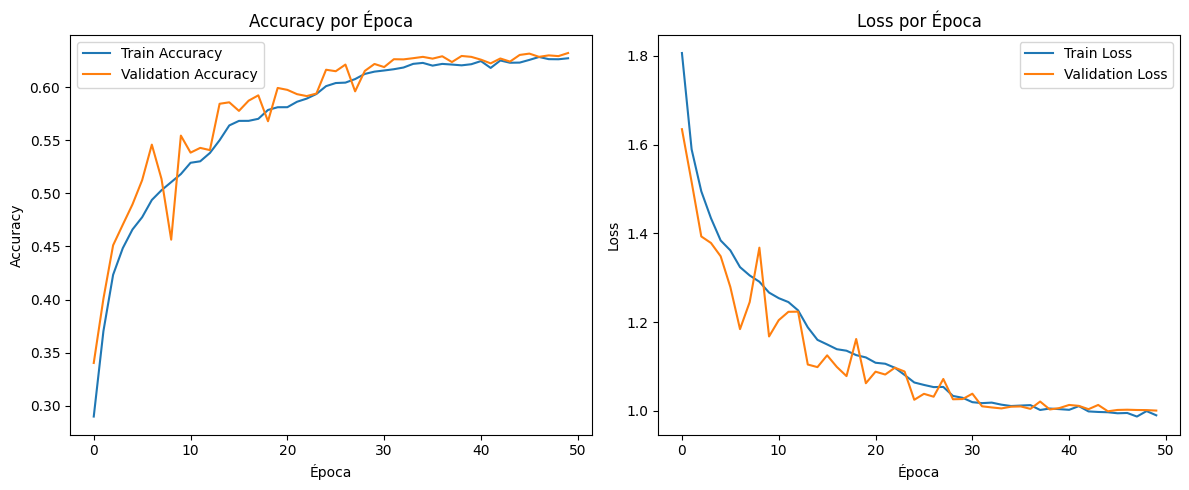
\includegraphics[width=0.9\textwidth]{img/accuracy-and-loss.png}
  \caption{Accuracy and loss per epoch during training}
  \label{fig:training-curves}
\end{figure}

\subsection{Confusion Matrix}

\begin{figure}[H]
  \centering
  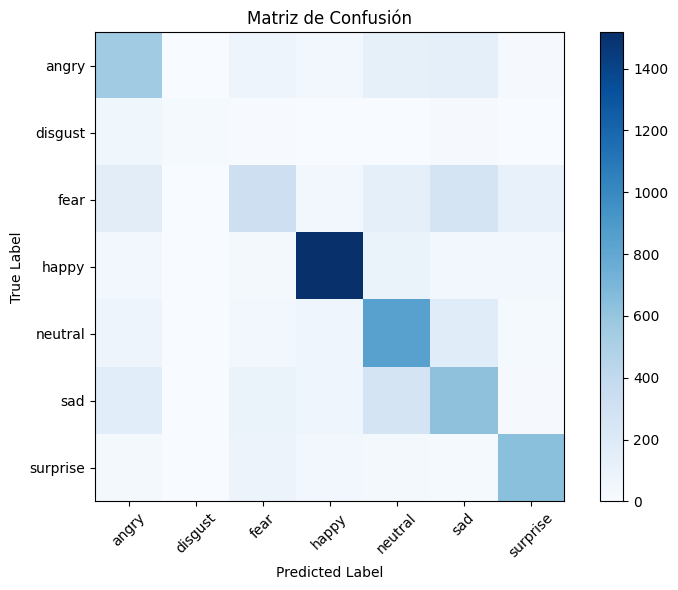
\includegraphics[width=0.65\textwidth]{img/confusion-matrix.png}
  \caption{Confusion matrix on the test set}
  \label{fig:confusion-matrix}
\end{figure}

% ─────────────────────────────────────────────
\section{Conclusions}

\subsection{Per-class performance}

The model achieved 63\% global accuracy on FER-2013, with highly variable per-class
performance. \textit{Happy} obtained the best result (F1 = 0.85), thanks to its highly
distinctive facial features. \textit{Surprise} also performed well (F1 = 0.76). In contrast,
\textit{disgust} achieved the lowest F1 (0.29) due to severe class imbalance: only 111 test
samples versus 1,774 for \textit{happy}.

\subsection{Most difficult emotions}

\textit{Fear} and \textit{sad} showed the weakest performance (F1 = 0.38 and 0.50,
respectively) for two complementary reasons: they share similar microexpressions --- downturned
mouth corners, tense eyebrows --- and class imbalance prevents the model from learning
sufficiently discriminative representations for \textit{disgust}.

\subsection{Relevance to the business case}

From the perspective of Sturm et al., the most important result is that \textit{happy} --- the
central emotion of the \textit{awe walks} protocol --- achieves F1 = 0.85, validating the
classifier for tracking longitudinal emotional trajectories. Strong performance on
\textit{surprise} (F1 = 0.76) is also relevant, since awe is frequently expressed as a
combination of happiness and surprise. The weaker performance on \textit{disgust} and
\textit{fear} is not a critical obstacle, as those emotions are not the primary hypotheses
of interest in the study.

\subsection{Proposed improvements}

\begin{enumerate}
  \item \textbf{Class balancing}: apply oversampling (SMOTE or aggressive augmentation) to
        minority classes, particularly \textit{disgust}.
  \item \textbf{Transfer learning}: replace the from-scratch architecture with a pre-trained
        backbone (VGG16, EfficientNetB0) and fine-tune. Such architectures reach 70--75\%
        accuracy on FER-2013.
  \item \textbf{Domain adaptation}: the study's corpus consists of selfies of older adults
        outdoors, a different domain from FER-2013 (laboratory/internet images). A domain
        adaptation cycle or fine-tuning on a small annotated sample would significantly
        improve real-world performance.
  \item \textbf{Per-class confidence thresholds}: in production, use differentiated thresholds
        to reject low-confidence predictions for classes such as \textit{fear} and
        \textit{disgust}.
\end{enumerate}

% ─────────────────────────────────────────────
\begin{thebibliography}{9}

\bibitem{sturm2022}
Sturm, V.\ E., Datta, S., Roy, A.\ R.\ K., Sible, I.\ J., Kosik, E.\ L., Veziris, C.\ R.,
Chow, T.\ E., Morris, N.\ A., Neuhaus, J., Kramer, J.\ H., Miller, B.\ L., Holley, S.\ R.,
\& Keltner, D.\ (2022).
\textit{Big smile, small self: Awe walks promote prosocial positive emotions in older adults.}
\textit{Emotion}, 22(5), 1044--1058.
\url{https://doi.org/10.1037/emo0000876}

\bibitem{fer2013}
Goodfellow, I.\ J., Erhan, D., Carrier, P.\ L., Courville, A., Mirza, M., Hamner, B.,
Cukierski, W., Tang, Y., Thaler, D., Lee, D.-H., Zhou, Y., Ramaiah, C., Feng, F., Li, R.,
Wang, X., Athanasakis, D., Shawe-Taylor, J., Milakov, M., Park, J., \ldots\ Bengio, Y.\
(2013).
\textit{Challenges in Representation Learning: A Report on Three Machine Learning Contests.}
arXiv:1307.0414.

\bibitem{fer2013-kaggle}
Sambare, M.\ (2020).
\textit{FER-2013} [Dataset].
Kaggle.
\url{https://www.kaggle.com/datasets/msambare/fer2013}

\bibitem{lecun1989}
LeCun, Y., Boser, B., Denker, J.\ S., Henderson, D., Howard, R.\ E., Hubbard, W.,
\& Jackel, L.\ D.\ (1989).
\textit{Backpropagation applied to handwritten zip code recognition.}
\textit{Neural Computation}, 1(4), 541--551.

\bibitem{tensorflow}
Abadi, M., et al.\ (2015).
\textit{TensorFlow: Large-scale machine learning on heterogeneous systems.}
\url{https://www.tensorflow.org}

\end{thebibliography}

\end{document}
